% !TeX spellcheck = en_GB
% !TEX TS-program = lualatex
% !TEX encoding = UTF-8 Unicode
\documentclass[aspectratio=169]{beamer}

%\setbeameroption{show notes}

\usetheme{metropolis}

\metroset{block=fill}

\title{Development of a Quantitative Comparison Tool for Plant Models }
\author{\textbf{Olivier Pieters}, Tom De Swaef and Francis wyffels}
\date{}
\institute{IDLab-AIRO -- Ghent University (UGent) -- imec\\
  Research Institute for Agriculture, Fisheries and Food (ILVO)}

\definecolor{input green}{HTML}{70dc70}
\definecolor{input ocre}{HTML}{ceb32a}
\definecolor{reservoir red}{HTML}{ff7d4d}
\definecolor{output pink}{HTML}{ef7bcc}
\definecolor{output blue}{HTML}{51a9ff}
\definecolor{light grey}{HTML}{afafaf}

\definecolor{nmse0}{HTML}{006eda}
\definecolor{nmse1}{HTML}{ffffff}

\usepackage{todonotes}

\usepackage{tikz}
\usetikzlibrary{matrix,calc,positioning,arrows.meta,backgrounds,matrix,fit,decorations.markings,3d,shapes}  

\tikzstyle{line} = [ultra thick]
\tikzstyle{<line>} = [line,{Latex[length=2mm, width=2mm]}-{Latex[length=2mm, width=2mm]}]
\tikzstyle{line>} = [line,-{Latex[length=2mm, width=2mm]}]
\tikzstyle{<line} = [line,{Latex[length=2mm, width=2mm]}-]


\usepackage{siunitx}

\tikzstyle{input node} = [draw,circle,minimum width=1cm,line width=0.3mm,fill=input green]
\tikzstyle{reservoir node} = [draw,circle,minimum width=0.5cm,line width=0.3mm,fill=reservoir red]
\tikzstyle{output node} = [draw,circle,minimum width=1cm,line width=0.3mm,fill=output blue]
\tikzstyle{box} = [dashed,line width=0.3mm]
\tikzstyle{box label} = [font=\Large]

\tikzstyle{model node}=[ultra thick, ellipse, minimum width=2cm, align=center]

\newcounter{resnode}

\usepackage{textcomp}

\usepackage{pgfplots}
\pgfplotsset{compat=1.16}
\usepgfplotslibrary{fillbetween,groupplots,units}

\makeatletter
\pgfplotsset{
  unit code/.code 2 args=
    \begingroup
    \protected@edef\x{\endgroup\si{#2}}\x
} 
\makeatother 

\usepackage{array}
\newcolumntype{L}[1]{>{\raggedright\let\newline\\\arraybackslash\hspace{0pt}}m{#1}}
\newcolumntype{C}[1]{>{\centering\let\newline\\\arraybackslash\hspace{0pt}}m{#1}}
\newcolumntype{R}[1]{>{\raggedleft\let\newline\\\arraybackslash\hspace{0pt}}m{#1}}

\usepackage{booktabs}

\pgfplotsset{perfplot/.style={matrix plot*,point meta=explicit,mesh/rows=10,mesh/ordering=y varies,}}

\usepackage{fontawesome5}

\newlength\nodesep
\setlength\nodesep{0.1cm}

\begin{document}

\begin{frame}[plain]
    \maketitle
    
    \begin{tikzpicture}[overlay,remember picture]
        \draw (current page.south east) ++(-0.5,0.5) node [anchor=south east] {\includegraphics[width=2cm]{figures/poster-AIRO-full-v1}};
    \end{tikzpicture}
\end{frame}

\begin{frame}{Plants Are Physical Reservoirs}
    \centering
    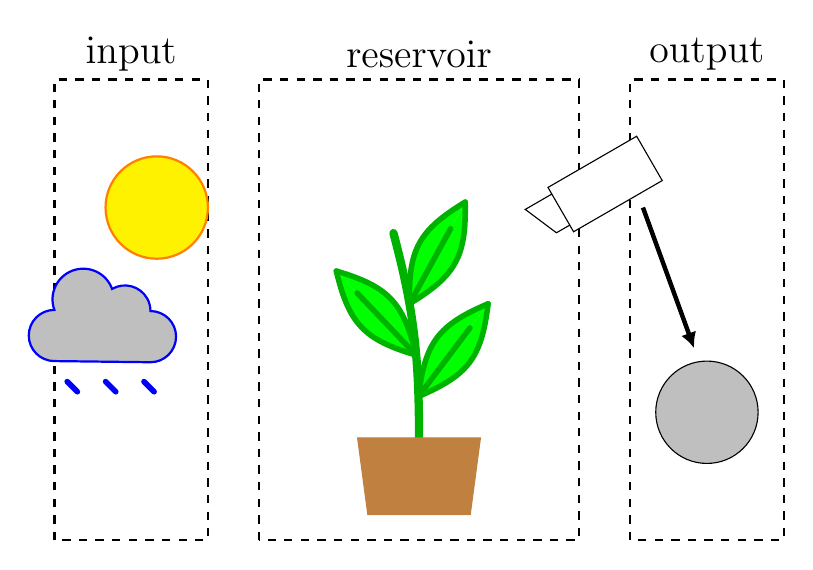
\begin{tikzpicture}[scale=0.65]
        % rectangles
        \draw[box] (-1.5,-4.5) rectangle (1.5,4.5);
        \draw[box] (2.5,-4.5) rectangle (8.75,4.5);
        \draw[box] (9.75,-4.5) rectangle (12.75,4.5);
        % draw rectangle labels
        \node[box label] at (0,5) {input};
        \node[box label] at (5.625,5) {reservoir};
        \node[box label] at (11.25,5) {output};
        
        % draw sun
        \draw[orange,fill=yellow,thick] (0.5,2) circle (1);
        % draw rays
        %\draw[fill=yellow,yellow,very thick] (0.5,2) ++(-60:1.2) ++(0.);
        %\draw[fill=yellow,yellow,very thick] (0.5,2) ++(-60:3.5) node (h3) {} arc (-60:-40:3.5) node (h4) {};
        % draw cloud
        \draw[blue,fill=gray!50!white,thick] (-1.5,-1) arc (270:90:0.5) arc (200:20:0.6) arc(120:0:0.5) arc (90:-90:0.5) -- cycle;
        % draw rain
        \foreach \x/\y in {-1.25/-1.4,-0.5/-1.4,0.25/-1.4} {
        	\draw[line width=2pt,blue,line cap=round] (\x,\y) -- ++(0.2,-0.2);
        }
        
        % draw plant
        \draw[postaction={decorate,
        	decoration={
        		markings,
        		mark=between positions 0.2 and 0.9 step 0.45 with {
        			\draw[line width=2pt,green!70!black,fill=green,line cap=round] (0,0) to[bend right,looseness=1.2] (1.15,-0.92);
        			\draw[line width=2pt,green!70!black,fill=green,line cap=round] (0,0) to[bend left,looseness=1.2] (1.15,-0.92);
        			\draw[line width=2pt,green!70!black,line cap=round] (0,0) -- (0.85,-0.68); 
        }}},
        postaction={decorate,
        	decoration={
        		markings,
        		mark=between positions 0.4 and 0.5 step 0.2 with {
        			\draw[line width=2pt,green!70!black,fill=green,line cap=round] (0,0) to[bend right,looseness=1.2] (1.15,0.92);
        			\draw[line width=2pt,green!70!black,fill=green,line cap=round] (0,0) to[bend left,looseness=1.2] (1.15,0.92);
        			\draw[line width=2pt,green!70!black,line cap=round] (0,0) -- (0.85,0.68); 
        		}
        }},
        green!70!black,line width=3pt,line cap=round] 
        (5.625,-2.5) to[out=90,in=-75] ++(-0.5,4);
        % draw pot
        \draw[brown,fill=brown] (5.625,-4) -- ++(-1,0) -- ++(-0.2,1.5) -- ++(2.4,0) -- ++(-0.2,-1.5) -- cycle;
        % draw camera
        \draw[rotate=30,fill=white] (8.25,-3) rectangle ++(2,1) (8.25,-2.85) -- ++(-0.3,0) -- ++(-0.3,0.7) -- ++(0.6,0) -- cycle;
        \draw[black,fill=gray!50!white] (11.25,-2) circle(1);
        \draw[line>] (10,2) -- (11,-0.75);
    \end{tikzpicture}
\end{frame}

\begin{frame}{Why is such a comparison relevant?}

    \onslide<1->{
    \begin{block}{Developers}
        For developers that want to know general properties of their models such as memory and non-linear dynamics
    \end{block}
    }
    
    \onslide<2->{
    \begin{block}{Users}
        Select the most appropriate of several available models
    \end{block}
    }
    
    \onslide<3->{
    \begin{alertblock}{Difficulty: no common paradigm or goal}
        Models have very different inner workings and their modelling goals also wildly differ.
    \end{alertblock}
    }

    \onslide<4->{
    \begin{exampleblock}{Reservoir computing}
        Our proposal: treat the model as a black box, and use a general computing framework to compare models
    \end{exampleblock}
    }
    
    %\textbf{\textrightarrow\ Reservoir computing}
    
\end{frame}


\begin{frame}{General ideal of reservoir computing: exploit rich dynamics}
    \centering
    
    \begin{tikzpicture}[scale=0.65]
    % input nodes
    \node[input node] at (0,1.25) (in0) {};
    \node[input node] at (0,-1.25) (in1) {};
    
    % reservoir nodes
    \foreach \x/\y in {3.5/0,4/2.25,5.5/1,6/-4,4/-2,6.25/-1.75,5.75/3.75,7.15/2.3,7.75/-0.35} {
    	\draw (\x,\y) node[reservoir node] (rn\the\value{resnode}) {};
    	\stepcounter{resnode}
    }
    
    % output nodes
    \foreach \y/\i in {2.5/0,0/1,-2.5/2} {
    	\node[output node] at (11.25,\y) (out\i) {};
    }
    
    % input arrows
    \foreach \i/\j in {0/0,0/6,0/4,1/3,1/0} {
    	\draw[line>] (in\i) -- (rn\j);
    }  
    
    % reservoir arrows
    \foreach \i/\j in {0/3,0/8,0/2,0/6,1/0,1/7,1/6,2/1,2/7,2/5,3/4,3/5,3/8,4/0,4/5,4/8,5/0,5/7,6/7,7/4,8/2,8/7} {
    	\draw[line>] (rn\i) -- (rn\j);
    }
    % bent arrows
    \draw[line>] (rn5) to[bend left] (rn2);
    \draw[line>] (rn6) to[out=180,in=110,looseness=1.3] (rn0);
    
    % output arrows
    \only<1>{
        \foreach \i/\j in {6/0,7/0,7/1,8/2,8/1,5/2,3/1} {
        	\draw[line>] (rn\i) -- (out\j);
        }
    }
    \only<2>{
        \foreach \i/\j in {6/0,7/0,7/1,8/2,8/1,5/2,3/1} {
        	\draw[line>,output pink] (rn\i) -- (out\j);
        }
    }
    \onslide<2->{
        \node[anchor=north] at (9.5,-4.75) {trained using linear regression};
    }
    
    % rectangles
    \draw[box] (-1.5,-4.5) rectangle (1.5,4.5);
    \draw[box] (2.5,-4.5) rectangle (8.75,4.5);
    \draw[box] (9.75,-4.5) rectangle (12.75,4.5);
    
    
    % draw rectangle labels
    \node[box label] at (0,5) {input};
    \node[box label] at (5.625,5) {reservoir};
    \node[box label] at (11.25,5) {output};
    \end{tikzpicture}
\end{frame}

\begin{frame}{Inspiration from compliant robotics and non-linear systems}
    \centering
    \begin{tikzpicture}
        \node[anchor=south west, inner sep=0] (image) at (0,0) {\includegraphics[width=0.7\linewidth]{figures/water-bucket}};
        \begin{scope}[x={(image.south east)},y={(image.north west)}]
            
            \onslide<2->{
            \draw[<line>,white] (0.225,0.225) -- ++(0,0.4);
            \draw[<line>,white] (0.725,0.225) -- ++(0,0.4);
            }
            
            \onslide<3->{
            \draw[reservoir red, ultra thick, rounded corners] (0.35,0.1) circle (15pt);
            }
%            \draw[reservoir red, ultra thick, rounded corners] (0.30,0.38) rectangle (0.37,0.46);
%            \draw[reservoir red, ultra thick, rounded corners] (0.75,0.39) rectangle (0.85,0.46);
%            
%            \draw[output pink, ultra thick, rounded corners] (0.45,0.31) circle (7.5pt);
%            \draw[output pink, ultra thick, rounded corners] (0.32,0.45) circle (7.5pt);
%            \draw[output pink, ultra thick, rounded corners] (0.77,0.43) circle (7.5pt);
        \end{scope}
        \draw (image.south west) node[below,anchor=north west] {\small\textit{Fernando et al. (2003)}};
    \end{tikzpicture}%
\end{frame}


\begin{frame}{Inspiration from compliant robotics and non-linear systems}
    \centering
    \begin{tikzpicture}
    \node[anchor=south west, inner sep=0] (image) at (0,0) {\includegraphics[width=0.75\linewidth]{figures/robots02}};
    \begin{scope}[x={(image.south east)},y={(image.north west)}]
        \onslide<2->{
        \draw[reservoir red, ultra thick, rounded corners] (0.43,0.24) rectangle (0.525,0.33);
        \draw[reservoir red, ultra thick, rounded corners] (0.30,0.38) rectangle (0.37,0.46);
        \draw[reservoir red, ultra thick, rounded corners] (0.75,0.39) rectangle (0.85,0.46);
        }
        
        \onslide<3->{
        \draw[output pink, ultra thick, rounded corners] (0.45,0.31) circle (7.5pt);
        \draw[output pink, ultra thick, rounded corners] (0.32,0.45) circle (7.5pt);
        \draw[output pink, ultra thick, rounded corners] (0.77,0.43) circle (7.5pt);
        }
    \end{scope}
    \end{tikzpicture}%
   
\end{frame}





\begin{frame}{General ideal of reservoir computing: exploit rich dynamics}
    \centering
    
    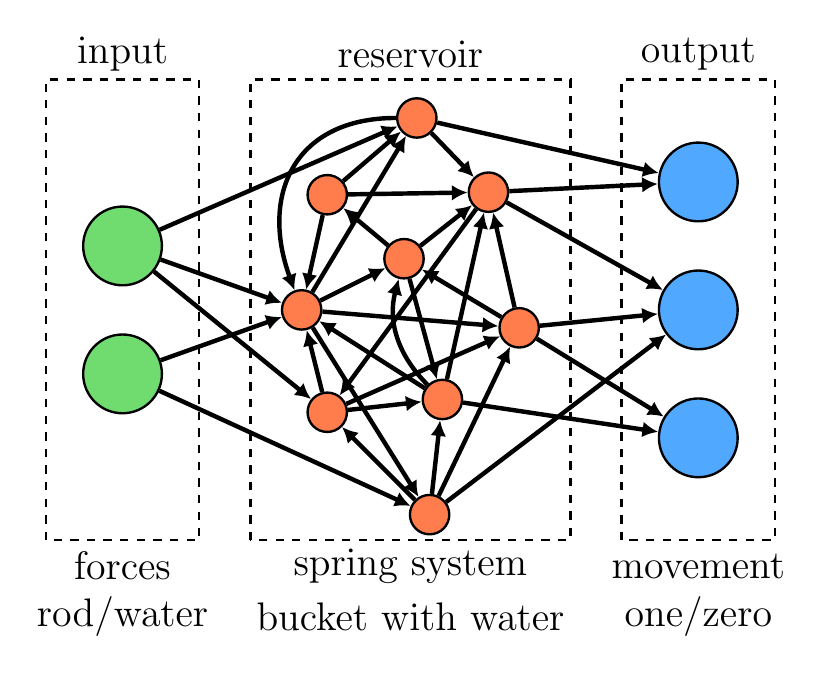
\begin{tikzpicture}[scale=0.65]
    % input nodes
    \node[input node] at (0,1.25) (in0) {};
    \node[input node] at (0,-1.25) (in1) {};
    
    % reservoir nodes
    \foreach \x/\y in {3.5/0,4/2.25,5.5/1,6/-4,4/-2,6.25/-1.75,5.75/3.75,7.15/2.3,7.75/-0.35} {
    	\draw (\x,\y) node[reservoir node] (rn\the\value{resnode}) {};
    	\stepcounter{resnode}
    }
    
    % output nodes
    \foreach \y/\i in {2.5/0,0/1,-2.5/2} {
    	\node[output node] at (11.25,\y) (out\i) {};
    }
    
    % input arrows
    \foreach \i/\j in {0/0,0/6,0/4,1/3,1/0} {
    	\draw[line>] (in\i) -- (rn\j);
    }  
    
    % reservoir arrows
    \foreach \i/\j in {0/3,0/8,0/2,0/6,1/0,1/7,1/6,2/1,2/7,2/5,3/4,3/5,3/8,4/0,4/5,4/8,5/0,5/7,6/7,7/4,8/2,8/7} {
    	\draw[line>] (rn\i) -- (rn\j);
    }
    % bent arrows
    \draw[line>] (rn5) to[bend left] (rn2);
    \draw[line>] (rn6) to[out=180,in=110,looseness=1.3] (rn0);
    
    % output arrows
    \foreach \i/\j in {6/0,7/0,7/1,8/2,8/1,5/2,3/1} {
    	\draw[line>] (rn\i) -- (out\j);
    }
    
    % rectangles
    \draw[box] (-1.5,-4.5) rectangle (1.5,4.5);
    \draw[box] (2.5,-4.5) rectangle (8.75,4.5);
    \draw[box] (9.75,-4.5) rectangle (12.75,4.5);
    
    
    % draw rectangle labels
    \node[box label] at (0,5) {input};
    \node[box label] at (5.625,5) {reservoir};
    \node[box label] at (11.25,5) {output};
    
    \onslide<2->{
        \node[box label] at (0,-5) {forces};
        \node[box label] at (5.625,-5) {spring system};
        \node[box label] at (11.25,-5) {movement};
        \node[box label] at (0,-6) {rod/water};
        \node[box label] at (5.625,-6) {bucket with water};
        \node[box label] at (11.25,-6) {one/zero};
    }
    \end{tikzpicture}
\end{frame}

\begin{frame}{Plant models are a set of reservoirs}
    \centering
    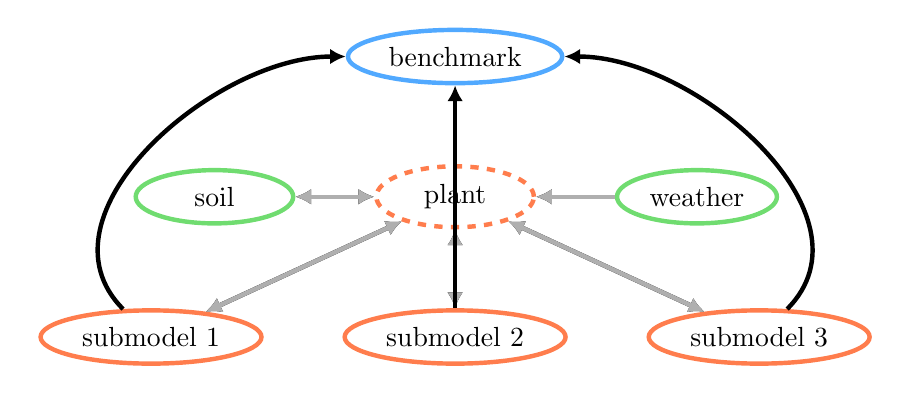
\begin{tikzpicture}
        \draw (0,0) node[model node,draw=reservoir red, dashed] (plant) {plant};
        \node[right=1 cm of plant, model node, draw=input green] (weather) {weather};
        \node[left=1 cm of plant, model node, draw=input green] (soil) {soil};
        \node[above=1 cm of plant, model node, draw=output blue] (benchmark) {benchmark};
        \node[below=1cm of plant,model node,draw=reservoir red] (sub2) {submodel 2};
        \node[left=1cm of sub2,model node,draw=reservoir red] (sub1) {submodel 1};
        \node[right=1cm of sub2,model node,draw=reservoir red] (sub3) {submodel 3};
        
        \onslide<1>{    mlineplot,
        \draw[<line>] (soil) -- (plant);
        \draw[line>] (weather) -- (plant);
        \draw[<line>] (plant) -- (sub1);
        \draw[<line>] (plant) -- (sub2);
        \draw[<line>] (plant) -- (sub3);
        }
        
        \onslide<2->{
            \draw[<line>,light grey] (soil) -- (plant);
            \draw[line>,light grey] (weather) -- (plant);
            \draw[<line>,light grey] (plant) -- (sub1);
            \draw[<line>,light grey] (plant) -- (sub2);
            \draw[<line>,light grey] (plant) -- (sub3);
            
            \draw[line>] (sub1) to[out=135,in=180] (benchmark);
            \draw[line>] (sub3) to[out=45,in=0] (benchmark);
            \draw[line>] (sub2) to (benchmark);
        }
         
        %\node 
    \end{tikzpicture}
\end{frame}

\begin{frame}{Benchmark tasks determine amount of memory and non-linearity}
    \begin{block}{Benchmark requirements}
        \begin{itemize}
            \item<1-> have some relation to the model
            \item<2-> varying memory properties
            \item<2-> varying non-linearity
            \item<3-> uniform metric to evaluate performance
        \end{itemize}
    \end{block}
\end{frame}

\begin{frame}{Our benchmark proposal}
    \begin{align}
        y[n+1] &= \dfrac{\tanh{\left(\alpha x[n]\right)}}{\tanh{\alpha}} - \sum_{i=0}^{d-1} h[i]y[n-i] \\
        h[i] &= \beta \exp\left[ -\left( i- \dfrac{d-1}{2}\right)^2 \right]
    \end{align}
    
    \centering
    
    \onslide<2->{
    \begin{tikzpicture}
        \begin{axis}[
            height=5cm,
            width=9cm,
            ylabel={$h[i]$},
            xlabel={$i$},
            grid=both,
        ]
            \addplot[
                ycomb,
                line width=1pt,
                mark=*,
                nmse0,
            ] table[x=x, y=h, col sep=comma] {data/filter_response.csv};
        \end{axis}
    \end{tikzpicture}
    }
\end{frame}

\begin{frame}{Effect of delay and non-linearity parameters on target}
    \centering
    \begin{tikzpicture}
        \begin{axis}[
            mlineplot,
            no marks,
            width=0.8\linewidth,
            height=4cm,
            xlabel={$x$},
            ylabel={$y$},
            legend style={at={(0,1)},anchor=north west},
            legend columns=2,
        ]
            \addplot+[line width=1pt] table[x=x, y=alpha0.1, col sep=comma] {data/non-linear_effect.csv};
            \addlegendentry{$\alpha=0.1$}
            \addplot+[line width=1pt] table[x=x, y=alpha0.5, col sep=comma] {data/non-linear_effect.csv};
            \addlegendentry{$\alpha=0.5$}
            %\addplot+[line width=1pt] table[x=x, y=alpha1.0, col sep=comma] {data/non-linear_effect.csv};
            %\addlegendentry{$\alpha=1.0$}
            \addplot+[line width=1pt] table[x=x, y=alpha2.0, col sep=comma] {data/non-linear_effect.csv};
            \addlegendentry{$\alpha=2.0$}
            \addplot+[line width=1pt] table[x=x, y=alpha5.0, col sep=comma] {data/non-linear_effect.csv};
            \addlegendentry{$\alpha=5.0$}
            \addplot+[line width=1pt] table[x=x, y=alpha10.0, col sep=comma] {data/non-linear_effect.csv};
            \addlegendentry{$\alpha=10.0$}
        \end{axis}
        \end{tikzpicture}
    \begin{tikzpicture}
        \begin{axis}[
        mlineplot,
        no marks,
        width=0.8\linewidth,
        height=4cm,
        xlabel={$n$},
        ylabel={$y$},
        ymin=-1.1,
        ymax=1.1,
        legend style={at={(0,0)},anchor=south west},
        legend columns=3,
        ]
            \addplot+[line width=1pt] table[x=t, y=x, col sep=comma] {data/delay_effect.csv};
            \addlegendentry{$x\ (d=0)$}
            \addplot+[line width=1pt] table[x=t, y=d1, col sep=comma] {data/delay_effect.csv};
            \addlegendentry{$d=1$}
            \addplot+[line width=1pt] table[x=t, y=d5, col sep=comma] {data/delay_effect.csv};
            \addlegendentry{$d=5$}
            \addplot+[line width=1pt] table[x=t, y=d20, col sep=comma] {data/delay_effect.csv};
            \addlegendentry{$d=20$}
            \addplot+[line width=1pt] table[x=t, y=d40, col sep=comma] {data/delay_effect.csv};
            \addlegendentry{$d=40$}
        \end{axis}
    \end{tikzpicture}
\end{frame}

\begin{frame}{Comparison metric: NMSE}
    \centering
    \begin{equation*}
        \text{NMSE} = \dfrac{\overline{\left(\hat{y} - y\right)^{2}}}{\text{var}{(y)}}
    \end{equation*}
    
    \begin{itemize}
        \item interesting range between 0 and 1.0
        \item NMSE of 0 is perfect prediction
        \item NMSE of 1.0 corresponds to mean prediction (baseline)
    \end{itemize}
\end{frame}

\begin{frame}{Data pipeline}
    \centering
    \begin{tikzpicture}[every node/.style={draw,rounded corners,thick}]
        \node (files) {\Large\faIcon[regular]{file-alt} \faIcon[regular]{file-alt} \faIcon[regular]{file-alt}};
        \node[below=5\nodesep of files] (table) {table with IO-data};
        \node[below=\nodesep of table] (benchmark) {O-data and benchmark data};
        \node[below left=\nodesep and \nodesep of benchmark] (train) {train data: \SI{60}{\percent}};
        \node[below right=\nodesep and \nodesep of benchmark] (test) {test data: \SI{40}{\percent}};
        \node[below=\nodesep of train] (std) {Standarision scaling};
        \node[below=\nodesep of std] (PCA) {PCA};
        \node[below=\nodesep of PCA] (LASSO) {LASSO};
        \node[below=3.5cm of table] (model) {optmised regressor};
        \node[below=5\nodesep of model] (NMSE) {NMSE score};
        \node[left=1cm of table] (params) {$\alpha$, $d$};
        
        \draw[line>] (files) -- (table) -- (benchmark);
        \draw[line>] (benchmark) -| (train);
        \draw[line>] (benchmark) -| (test);
        \draw[line] (train) -- (std) -- (PCA) -- (LASSO);
        \draw[line>] (LASSO) |- (model);
        \draw[line>] (test) |- (model);
        \draw[line>] (model) -- (NMSE);
        
        \draw[line>] (params) -| ($0.1*(benchmark.north east)+0.9*(benchmark.north west)$);
        
        \only<1>{
            \node[reservoir red] (files) {\Large\faIcon[regular]{file-alt} \faIcon[regular]{file-alt} \faIcon[regular]{file-alt}};
            \node[below=5\nodesep of files,reservoir red] (table) {table with IO-data};
            \node[below=\nodesep of table,reservoir red] (benchmark) {O-data and benchmark data};
            \node[left=1cm of table,reservoir red] (params) {$\alpha$, $d$};
        }
        \only<2>{
            \node[below left=\nodesep and \nodesep of benchmark,reservoir red] (train) {train data: \SI{60}{\percent}};
            \node[below right=\nodesep and \nodesep of benchmark,reservoir red] (test) {test data: \SI{40}{\percent}};
        }
        \only<3>{
            \node[below=\nodesep of train,reservoir red] (std) {Standarision scaling};
            \node[below=\nodesep of std,reservoir red] (PCA) {PCA};
            \node[below=\nodesep of PCA,reservoir red] (LASSO) {LASSO};
        }
        \only<4>{
            \node[below=3.5cm of table,reservoir red] (model) {optmised regressor};
            \node[below=5\nodesep of model,reservoir red] (NMSE) {NMSE score};
        }
    \end{tikzpicture}
\end{frame}

\begin{frame}{Example figure}
    \centering
    \begin{tikzpicture}
        \begin{axis}[
            xlabel={delay $d$},
            ylabel={$\log\alpha$},
            colorbar,
            colormap={maskimage}{color(0)=(nmse0); color(1)=(nmse1)},
            xmin=-2.5,
            xmax=47.5,
            ymin=-3.75,
            ymax=1.25,
        ]
            \onslide<1->{
            \addplot[
                matrix plot*,
                point meta=explicit,
            ] table [meta=v] {data/simple-plot.dat};
            }
            
            \draw (axis cs:0,-3.5)  coordinate (baseline);
            \draw (axis cs:40,-3.5) coordinate (end1);
            \draw (axis cs:0,0.5) coordinate (end2);
            \draw (axis cs:40,0.5) coordinate (end3);
        \end{axis}
        
        \only<2>{
            \fill (baseline) circle (2pt);
            \draw (baseline) node[above right] {\textbf{baseline}};
        }
        \onslide<3->{
            \draw[line>] (baseline) -- (end1) node[anchor=south east] {\textbf{increase delay}};
        }
        \onslide<4->{
            \draw[line>,align=left] (baseline) -- (end2) node[anchor=west] {\textbf{increase}\\\textbf{non-linearity}};
        }
        \onslide<5->{
            \draw[line>,align=right] (baseline) -- (end3) node[pos=0.5,above,sloped] {\textbf{increased difficulty}};
        }
    \end{tikzpicture}
\end{frame}

\begin{frame}{Case study: WheatFSPM}
    \centering
    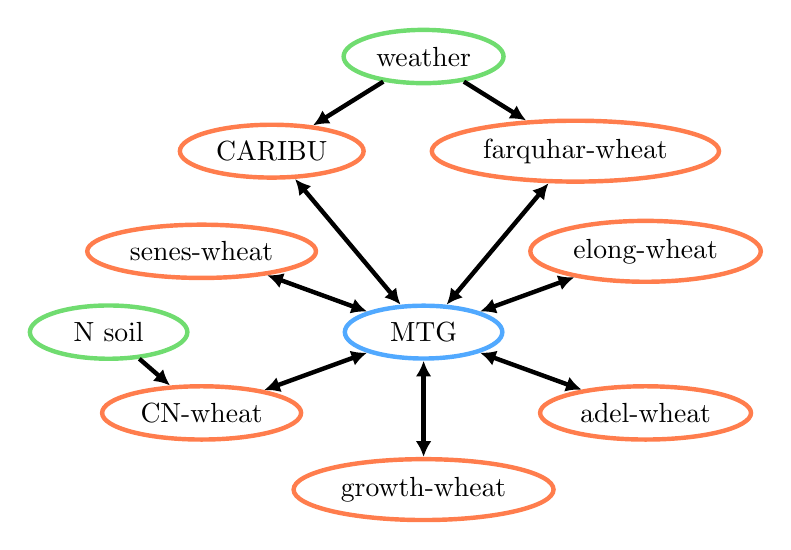
\begin{tikzpicture}
        \def\fspmR{3}
        \node[model node,draw=output blue] (mtg) {MTG};
        \draw (mtg) ++(20:\fspmR) node[model node,draw=reservoir red] (elong-wheat) {elong-wheat};
        \draw (mtg) ++(50:\fspmR) node[model node,draw=reservoir red] (farquhar-wheat) {farquhar-wheat};
        \draw (mtg) ++(130:\fspmR) node[model node,draw=reservoir red] (caribu) {CARIBU};
        \draw (mtg) ++(160:\fspmR) node[model node,draw=reservoir red] (senes-wheat) {senes-wheat};
        \draw (mtg) ++(200:\fspmR) node[model node,draw=reservoir red] (CN-wheat) {CN-wheat};
        \draw (mtg) ++(270:2) node[model node,draw=reservoir red] (growth-wheat) {growth-wheat};
        \draw (mtg) ++(340:\fspmR) node[model node,draw=reservoir red] (adel-wheat) {adel-wheat};
        
        \draw (mtg) ++(90:3.5) node[model node,draw=input green] (weather) {weather};
        \draw (mtg) ++(180:4) node[model node,draw=input green] (soil) {N soil};
        
        \draw[<line>] (mtg) -- (elong-wheat);
        \draw[<line>] (mtg) -- (farquhar-wheat);
        \draw[<line>] (mtg) -- (caribu);
        \draw[<line>] (mtg) -- (senes-wheat);
        \draw[<line>] (mtg) -- (CN-wheat);
        \draw[<line>] (mtg) -- (growth-wheat);
        \draw[<line>] (mtg) -- (adel-wheat);
        
        \draw[line>] (weather) -- (caribu);
        \draw[line>] (weather) -- (farquhar-wheat); 
        \draw[line>] (soil) -- (CN-wheat); 
        
    \end{tikzpicture}
    % adopted from Adapted from Gauthier et al. (2020)
\end{frame}

\begin{frame}{WheatFSPM reservoir overview}
    \centering
    \begin{tabular}{lL{7cm}}
    \toprule
    abbreviation & description \\
    \midrule
    photo & photosynthesis and respiration outputs\\
    E & energy related parameters (fructose, sucrose, starch)\\
    proteins & protein outputs\\
    N & nitrogen outputs\\
    str. & structural outputs (mass, lengths) \\
    cytokinins & cytokinin outputs\\
    \bottomrule
    \end{tabular}
\end{frame}

\begin{frame}[fragile]
\makebox[\textwidth][c]{%
\def\df{data/vis-data-1plants.dat}
\begin{tikzpicture}
    \begin{groupplot}[
        width = 3cm,
        height = 3cm,
        group style={
          group size=6 by 5,
          horizontal sep=0pt,
          vertical sep=0pt,
          ylabels at=edge left,
          xlabels at=edge bottom,
          xticklabels at=edge bottom,
          yticklabels at=edge left,
          group name=env,},
        %enlargelimits=false,
        xtick={10,30},
        colormap={maskimage}{color(0)=(nmse0); color(1)=(nmse1)},
        axis on top=true,
        xlabel={$d$ [\si{\hour}]},
        %x unit={\hour},
        ylabel={$\log \alpha$},
        y unit={},
        xmin=-2.5,
        xmax=47.5,
        ymin=-3.75,
        ymax=1.75,
        point meta min=0.0,
        point meta max=1.0,
    ]
    
    \pgfplotsinvokeforeach{respiration+photosynthesis-air_temperature,sucrose+fructan+starch-air_temperature,proteins-air_temperature,N-air_temperature,structure-air_temperature}{%
        \nextgroupplot[]
        \addplot [perfplot] table [meta=#1] {\df};
    }
    
    \nextgroupplot[
        colorbar,
        every colorbar/.append style={
            height=5*\pgfkeysvalueof{/pgfplots/parent axis height}+
                \pgfkeysvalueof{/pgfplots/group/vertical sep},
            },
        colorbar style={
        name=clb,
        },
    ]
    \addplot [perfplot] table [meta=cytokinins-air_temperature] {\df};
    
    
    \pgfplotsinvokeforeach{cytokinins-air_temperature,respiration+photosynthesis-PARi,sucrose+fructan+starch-PARi,proteins-PARi,N-PARi,structure-PARi,cytokinins-PARi,respiration+photosynthesis-soil_temperature,sucrose+fructan+starch-soil_temperature,proteins-soil_temperature,N-soil_temperature,structure-soil_temperature,cytokinins-soil_temperature,respiration+photosynthesis-humidity,sucrose+fructan+starch-humidity,proteins-humidity,N-humidity,structure-humidity,cytokinins-humidity,respiration+photosynthesis-Wind,sucrose+fructan+starch-Wind,proteins-Wind,N-Wind,structure-Wind,cytokinins-Wind}{%
        \nextgroupplot[]
        \addplot [perfplot] table [meta=#1] {\df};
    }
  
    \end{groupplot}
    
    \node[below=0.2cm of clb.south,anchor=north] {NMSE};
    
    \begin{scope}[every node/.style={
        %text width=1cm,
        anchor=south,
        text depth=5pt,
        align=center}
    ]
        \node at (env c1r1.north) {\large photo};
        \node at (env c2r1.north) {\large E};
        \node at (env c3r1.north) {\large proteins};
        \node at (env c4r1.north) {\large N};
        \node at (env c5r1.north) {\large str.};
        \node at (env c6r1.north) {\large cytokinins};
    \end{scope}
    \begin{scope}[every node/.style={
        %text width=1cm,
        anchor=east,
        text depth=5pt,
        align=right}
    ]
        \node at ($(env c1r1.west)+(-1.5,0)$) {\large T\textsubscript{air}};
        \node at ($(env c1r2.west)+(-1.5,0)$) {\large PAR};
        \node at ($(env c1r3.west)+(-1.5,0)$) {\large T\textsubscript{soil}};
        \node at ($(env c1r4.west)+(-1.5,0)$) {\large RH};
        \node at ($(env c1r5.west)+(-1.5,0)$) {\large wind};
    \end{scope}
    
    \node[below left=0.1cm and 0.1cm of env c1r5,anchor=north east,align=center] {\textbf{1 plant}};
\end{tikzpicture}%
}
\end{frame}

\begin{frame}[fragile]
\makebox[\textwidth][c]{%
\def\df{data/vis-data-10plants.dat}
\begin{tikzpicture}
    \begin{groupplot}[
        width = 3cm,
        height = 3cm,
        group style={
          group size=6 by 5,
          horizontal sep=0pt,
          vertical sep=0pt,
          ylabels at=edge left,
          xlabels at=edge bottom,
          xticklabels at=edge bottom,
          yticklabels at=edge left,
          group name=env,},
        %enlargelimits=false,
        xtick={10,30},
        colormap={maskimage}{color(0)=(nmse0); color(1)=(nmse1)},
        axis on top=true,
        xlabel={$d$ [\si{\hour}]},
        %x unit={\hour},
        ylabel={$\log \alpha$},
        y unit={},
        xmin=-2.5,
        xmax=47.5,
        ymin=-3.75,
        ymax=1.75,
        point meta min=0.0,
        point meta max=1.0,
    ]
    
    \pgfplotsinvokeforeach{respiration+photosynthesis-air_temperature,sucrose+fructan+starch-air_temperature,proteins-air_temperature,N-air_temperature,structure-air_temperature}{%
        \nextgroupplot[]
        \addplot [perfplot] table [meta=#1] {\df};
    }
    
    \nextgroupplot[
        colorbar,
        every colorbar/.append style={
            height=5*\pgfkeysvalueof{/pgfplots/parent axis height}+
                \pgfkeysvalueof{/pgfplots/group/vertical sep},
            },
        colorbar style={
        name=clb,
        },
    ]
    \addplot [perfplot] table [meta=cytokinins-air_temperature] {\df};
    
    
    \pgfplotsinvokeforeach{cytokinins-air_temperature,respiration+photosynthesis-PARi,sucrose+fructan+starch-PARi,proteins-PARi,N-PARi,structure-PARi,cytokinins-PARi,respiration+photosynthesis-soil_temperature,sucrose+fructan+starch-soil_temperature,proteins-soil_temperature,N-soil_temperature,structure-soil_temperature,cytokinins-soil_temperature,respiration+photosynthesis-humidity,sucrose+fructan+starch-humidity,proteins-humidity,N-humidity,structure-humidity,cytokinins-humidity,respiration+photosynthesis-Wind,sucrose+fructan+starch-Wind,proteins-Wind,N-Wind,structure-Wind,cytokinins-Wind}{%
        \nextgroupplot[]
        \addplot [perfplot] table [meta=#1] {\df};
    }
  
    \end{groupplot}
    
    \node[below=0.2cm of clb.south,anchor=north] {NMSE};
    
    \begin{scope}[every node/.style={
        %text width=1cm,
        anchor=south,
        text depth=5pt,
        align=center}
    ]
        \node at (env c1r1.north) {\large photo};
        \node at (env c2r1.north) {\large E};
        \node at (env c3r1.north) {\large proteins};
        \node at (env c4r1.north) {\large N};
        \node at (env c5r1.north) {\large str.};
        \node at (env c6r1.north) {\large cytokinins};
    \end{scope}
    \begin{scope}[every node/.style={
        %text width=1cm,
        anchor=east,
        text depth=5pt,
        align=right}
    ]
        \node at ($(env c1r1.west)+(-1.5,0)$) {\large T\textsubscript{air}};
        \node at ($(env c1r2.west)+(-1.5,0)$) {\large PAR};
        \node at ($(env c1r3.west)+(-1.5,0)$) {\large T\textsubscript{soil}};
        \node at ($(env c1r4.west)+(-1.5,0)$) {\large RH};
        \node at ($(env c1r5.west)+(-1.5,0)$) {\large wind};
    \end{scope}
    
    \node[below left=0cm and 0cm of env c1r5,anchor=north east,align=center] {\textbf{10 plants, different}\\\textbf{arch., imperfect sowing}};
\end{tikzpicture}%
}
\end{frame}

\begin{frame}{Conclusion}
    Applied reservoir computing to FSPM plant models.
    
    Benchmark estimates both non-linear and memory properties of plant models.
    
    Benchmark enables comparison between models relative to certain input vectors.
    
    Benchmark's stability should be improved
\end{frame}

\begin{frame}{Source Code on GitHub}
    \begin{center}
        Code and data on GitHub:
        
        {\small \url{https://github.com/opieters/plant_model_comparison}}
        
        \vspace{0.5cm}
        
        \href{mailto:olivier.pieters@ugent.be}{olivier.pieters@ugent.be}
        
        \vspace{\fill}
        
        Presentation and figures: CC-BY-SA 4.0
        
        \includegraphics[width=2cm]{figures/CC-BY-SA}
    \end{center}
\end{frame}

\end{document}